\documentclass[runningheads,a4paper]{llncs2e/llncs}
\usepackage{makeidx}

\usepackage{amssymb}
\setcounter{tocdepth}{3}
\usepackage{graphicx}
\usepackage{url}
\usepackage{times}
%\usepackage{titlesec}
\usepackage{clrscode4e}
\usepackage{supertech}
\usepackage{pgfplots}

\let\epsilon=\varepsilon

\begin{document}


\frontmatter
\pagestyle{headings}

%\tableofcontents
%
\mainmatter              % start of the contributions
%
\title{Bigger and Faster Data-graph Computations for Physical Simulations}
%
\titlerunning{Bigger and Faster}  % abbreviated title (for running head)
%                                     also used for the TOC unless
%                                     \toctitle is used
%
\author{Predrag Gruevski, William Hasenplaugh, \and James J. Thomas}
%
\authorrunning{Gruevski et al.} % abbreviated author list (for running head)
%
%%%% list of authors for the TOC (use if author list has to be modified)
\tocauthor{Predrag Gruevski, William Hasenplaugh, and James J. Thomas}
%
\institute{Massachusetts Institute of Technology\\
Cambridge, MA 02139, USA\\
\{predrag, whasenpl, jjthomas\}@mit.edu\\
\url{http://toc.csail.mit.edu/}}

\maketitle

\punt{
Outline:
\begin{itemize}
\item Introduction
	\item Motivation and Problem Definition
	\item DGC
		\begin{itemize}
		\item Definition
		\item Scheduling algorithms
		\item Qualitative rationale for cache perils of chromatic and potential benefit to dag scheduling
		\end{itemize}
	\item Simit
		\begin{itemize}
		\item High-level description
		\item How to represent graph as a DGC
		\end{itemize}
	\item Hilbert 
		\begin{itemize}
		\item Quick qualitative overview of the cache behavior of our approach 
		\item Ditto for partitioning 
		\end{itemize}
	\item Paper organization
\item Multi-core Cache Performance
	\begin{itemize}
	\item Define hilbert priority function and general work flow of ordering algorithm
	\item Show distribution of vertex ID distance between every pair of neighbors w/ and w/o Hilbert ordering
	\item Give rationale for why it exhibits good cache behavior (perhaps show Theorem w/o proof)
	\end{itemize}
\item Multi-core Experimental Results
	\begin{itemize}
	\item Define experimental methodology
	\item Give results
	\end{itemize}
\item Distributed Memory
	\begin{itemize}
	\item Rationale for why Hilbert ordering should be good for distributed memory
	\item Show fraction of edges that cross partitions w/ and w/o Hilbert ordering
	\end{itemize}
\item Distributed Memory Experimental Results
	\begin{itemize}
	\item Define experimental methodology
	\item Give results
	\end{itemize}
\end{itemize}
}

% \begin{itemize}
% \item Describe BFS and why the data-access pattern is problematic
% \item Describe software prefetching strategy and sw changes
% \item Go over measurements and perf stat observations (e.g. inst / edge and TLB misses)
% \item Describe phenomenon of page walkers dominating performance and explain why sw prefetching still helps (due to limited OoO window size)
% \item Go over large page measurements and explain why performance improves so much
% \end{itemize}

\begin{abstract}
\label{abstract}
% We investigate the problem of executing physical simulations 
% efficiently on a cluster of computers. We cast the problem 
% as a data-graph computation in the style of GraphLab, where 
% vertices represent points in a physical mesh and edges connect 
% nearby vertices. Taking advantage of the special properties 
% of mesh graphs, including the locality of edges, we devise 
% and evaluate schemes for partioning such graphs across a 
% cluster of computers to minimize communication and for 
% performing vertex updates on individual machines with high 
% cache locality and parallelism.
We investigate the problem of implementing the physical simulations
specified in the domain-specific language Simit as a \defn{data-graph
computation}.
{Data-graph computations} consist of a graph $G=(V,E)$, where
each vertex has data associated with it, and an update function 
which is applied to each vertex, taking as inputs the neighboring 
vertices.  \proc{Prism} is a framework for executing data-graph
computations in shared memory using a scheduling technique called 
\emph{chromatic scheduling}, where a coloring of the input graph
is used to parcel out batches of independent work, sets of 
vertices with a common color, while preserving
determinism.  An alternative scheduling approach is \emph{priority-dag
scheduling} where a priority function $\rho$ mapping each vertex $v \in V$
to a real number is used to orient the edges from low to high priority and
and thus generate a dag.  We propose to extend \proc{Prism} in two primary
ways.  First, we will extend it to use distributed memory to enable
problem sizes many orders of magnitude larger than the current 
implementation using a graph partitioning approach which minimizes
the number of edges that cross distributed memory nodes.  
Second, we will replace the chromatic scheduler in
\proc{Prism} with a priority-dag scheduler and a priority function 
which generates a cache-efficient traversal of the vertices when the
input graph is locally connected and embeddable in a low-dimensional 
space.  This subset of graphs is important for the physical simulations
generated by the language Simit.  
\end{abstract}

\section{Introduction}
\label{sec:intro}



\begin{figure}[!t]
\centering
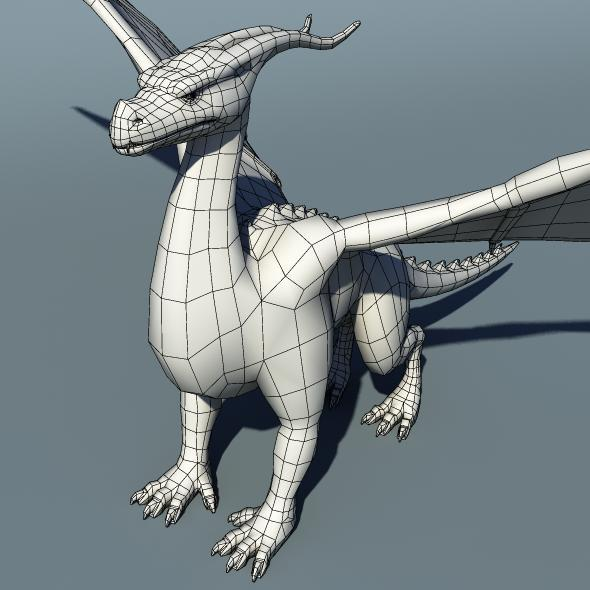
\includegraphics[width=2.5in]{dragon}
\caption{A mesh graph where lines correspond to edges and intersections of lines correspond to vertices.}
\label{fig:mesh}
\end{figure}

\subheading{Contributions}

We anticipate contributing a new technique for and a well-engineered
implementation of a cache-efficient data-graph computation using
priority-dag scheduling.  In addition, our implementation will support
extremely large simulations on distributed-memory clusters.  Both
of these contributions are high-impact features for the customers
of Simit, for which \proc{Prism} will be the new backend for multi-cores
and clusters of multi-cores.  We have some initial exploratory code
of priority functions (e.g. BFS depth, color).  

\subheading{Task Breakdown}

James and Predrag will extend \proc{Prism} to support data reshuffling
based on a priority per vertex.  Initially, this will be a standalone
utility that reads a graph file, reorders the vertices and writes out
the shuffled file.  

Will and Mohsen will engineer the MPI support for distributed memory,
including support for distributed data loading.

\subheading{Issues}

We descoped our project to focus on being a good back-end for Simit, which
works on graphs of physical simulations.  This means ditching the investigation
of software prefetching and static assignment of vertices to processors.
However, our new focus has allowed us to do something more elegant, essentially
a cache-oblivious scheduling algorithm for data-graph computations on graphs
of physical simulations.

\section{Introduction}
\label{sec:intro}

This section introduces the problem of deterministically scheduling data-graph
computations while preserving good cache efficiency on the special subset of graphs
that are locally connected and embeddable in a low-dimensional space.  

\subsection{Cache Efficiency Perils}

This section will demonstrate the cache efficiency issues inherent in chromatic
scheduling and dag-scheduling with a poor priority function.  

\subsection{Distributed Memory}

In this section, we will discuss
the challenges in extending the implementation of \proc{Prism} to support
distributed memory. 

\section{Fast Execution on Individual Machines}
\label{sec:multicore}


\subsection{Space-filling Curves}

Outline:
\begin{itemize}
\item Define hilbert priority function and general work flow of ordering algorithm
\item Show distribution of vertex ID distance between every pair of neighbors w/ and w/o Hilbert ordering
\item Give rationale for why it exhibits good cache behavior (perhaps show Theorem w/o proof)
\end{itemize}




In this section, we will describe the rationale behind using the
Hilbert space-filling curve as a way of mapping an $N$-dimensional
space onto the real line, specifically to use this mapping as a
priority function for the priority-dag scheduler in \proc{Prism}.
We will present event counters (e.g. cache misses, TLB misses etc.), 
measured performance and span for three serial experiments on the same
set of graphs: chromatic scheduling, priority-dag scheduling with
a random priority function and priority-dag scheduling with a
Hilbert curve priority function.  

\begin{figure}[h]
\centering
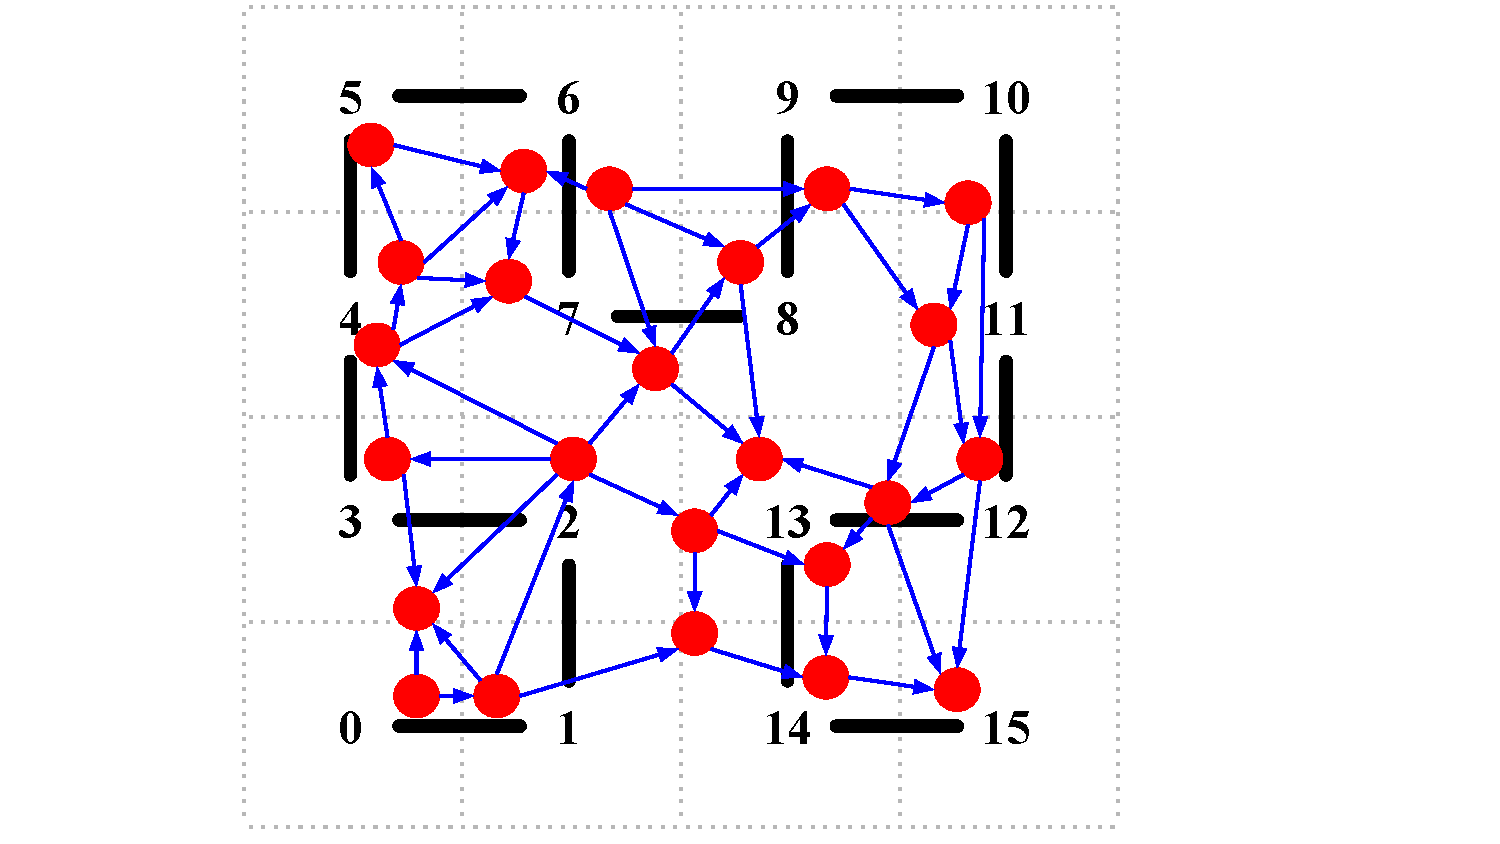
\includegraphics[width=5in]{figures/hilbert_priority_function.pdf}
\caption{Example of how a locally-connected graph in 2 dimensions
is mapped to a dag via the Hilbert priority function.  Each
vertex is mapped to its closest grid point in the discretized
Hilbert curve.  Among vertices mapping to the same Hilbert grid
point, ties are broken randomly.}
\label{fig:hilbert_priority}
\end{figure}


\begin{figure}[h]
\centering
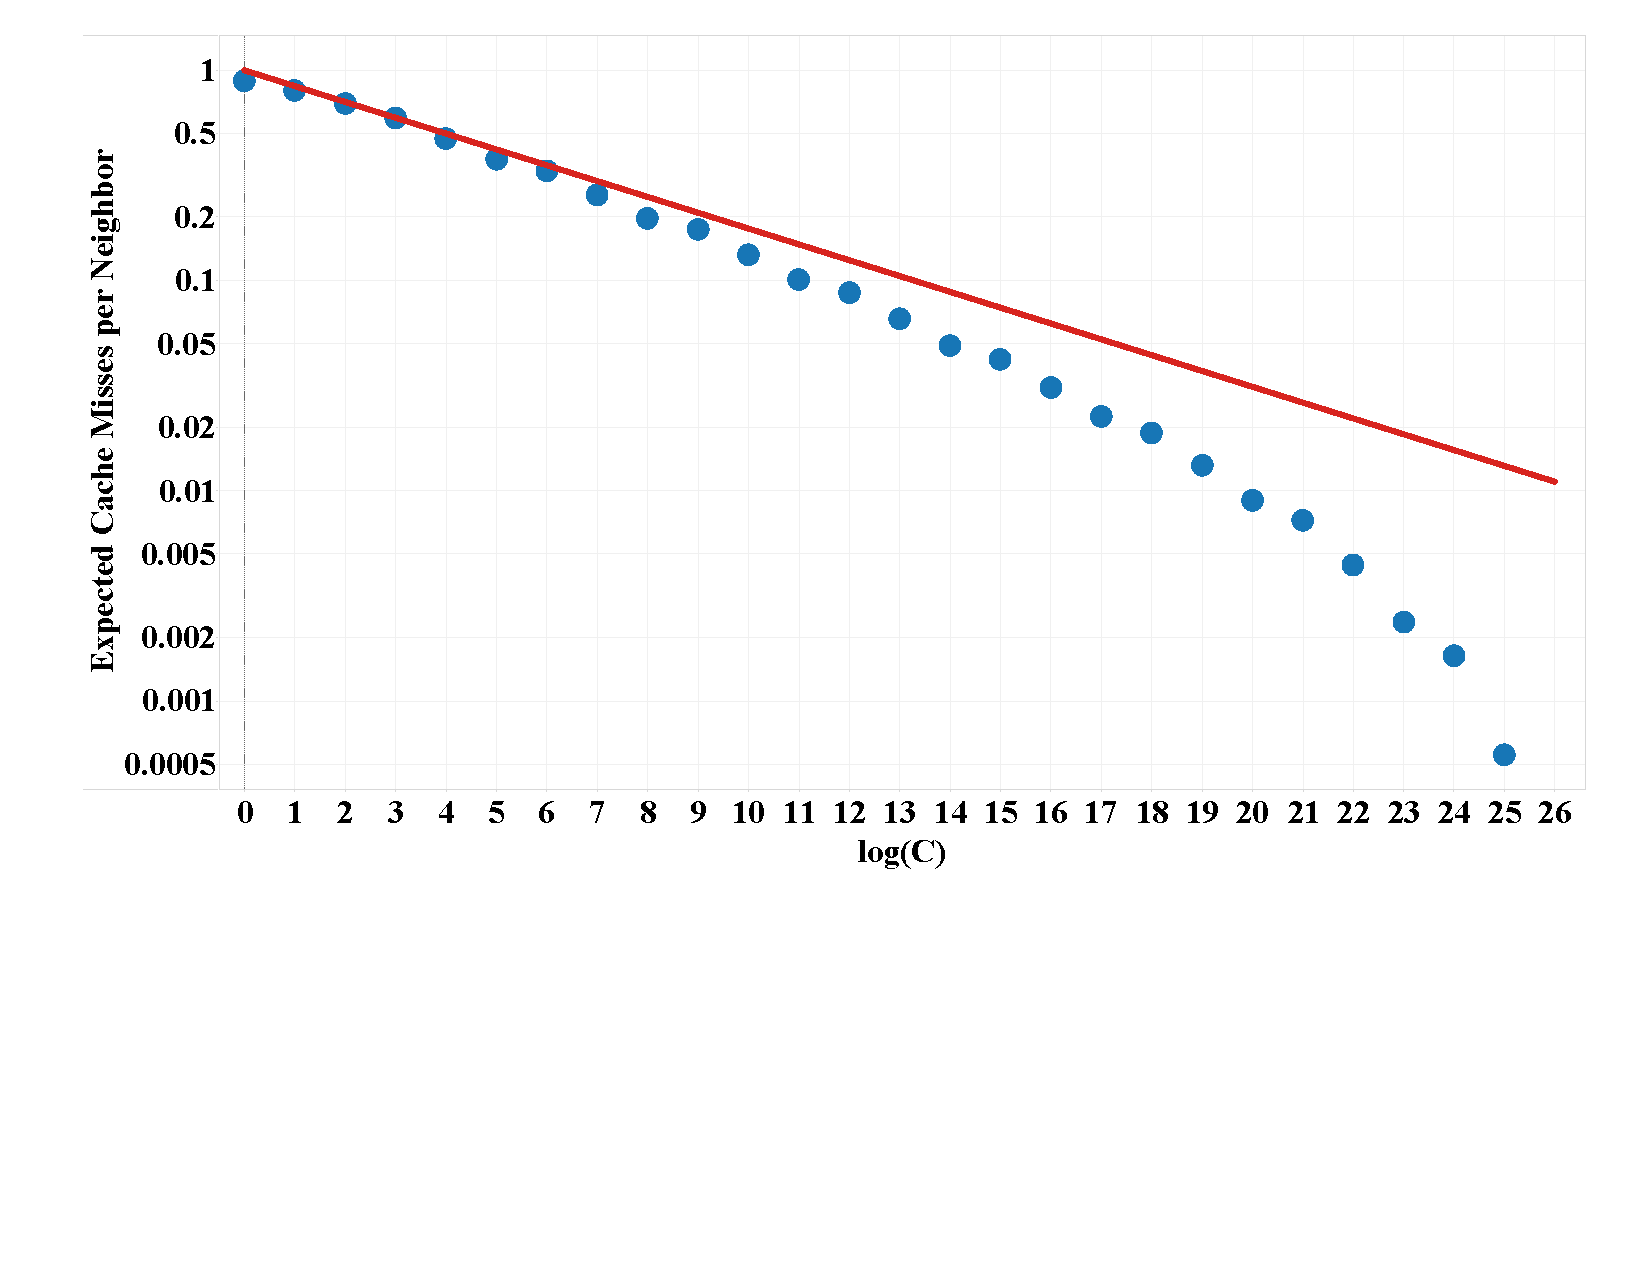
\includegraphics[width=5in,clip,trim=1cm 6cm 0 0]{figures/miss_rate_curve.pdf}
\caption{Miss rate curve...}
\label{fig:miss_rate_curve}
\end{figure}

\begin{figure}[h]
\centering
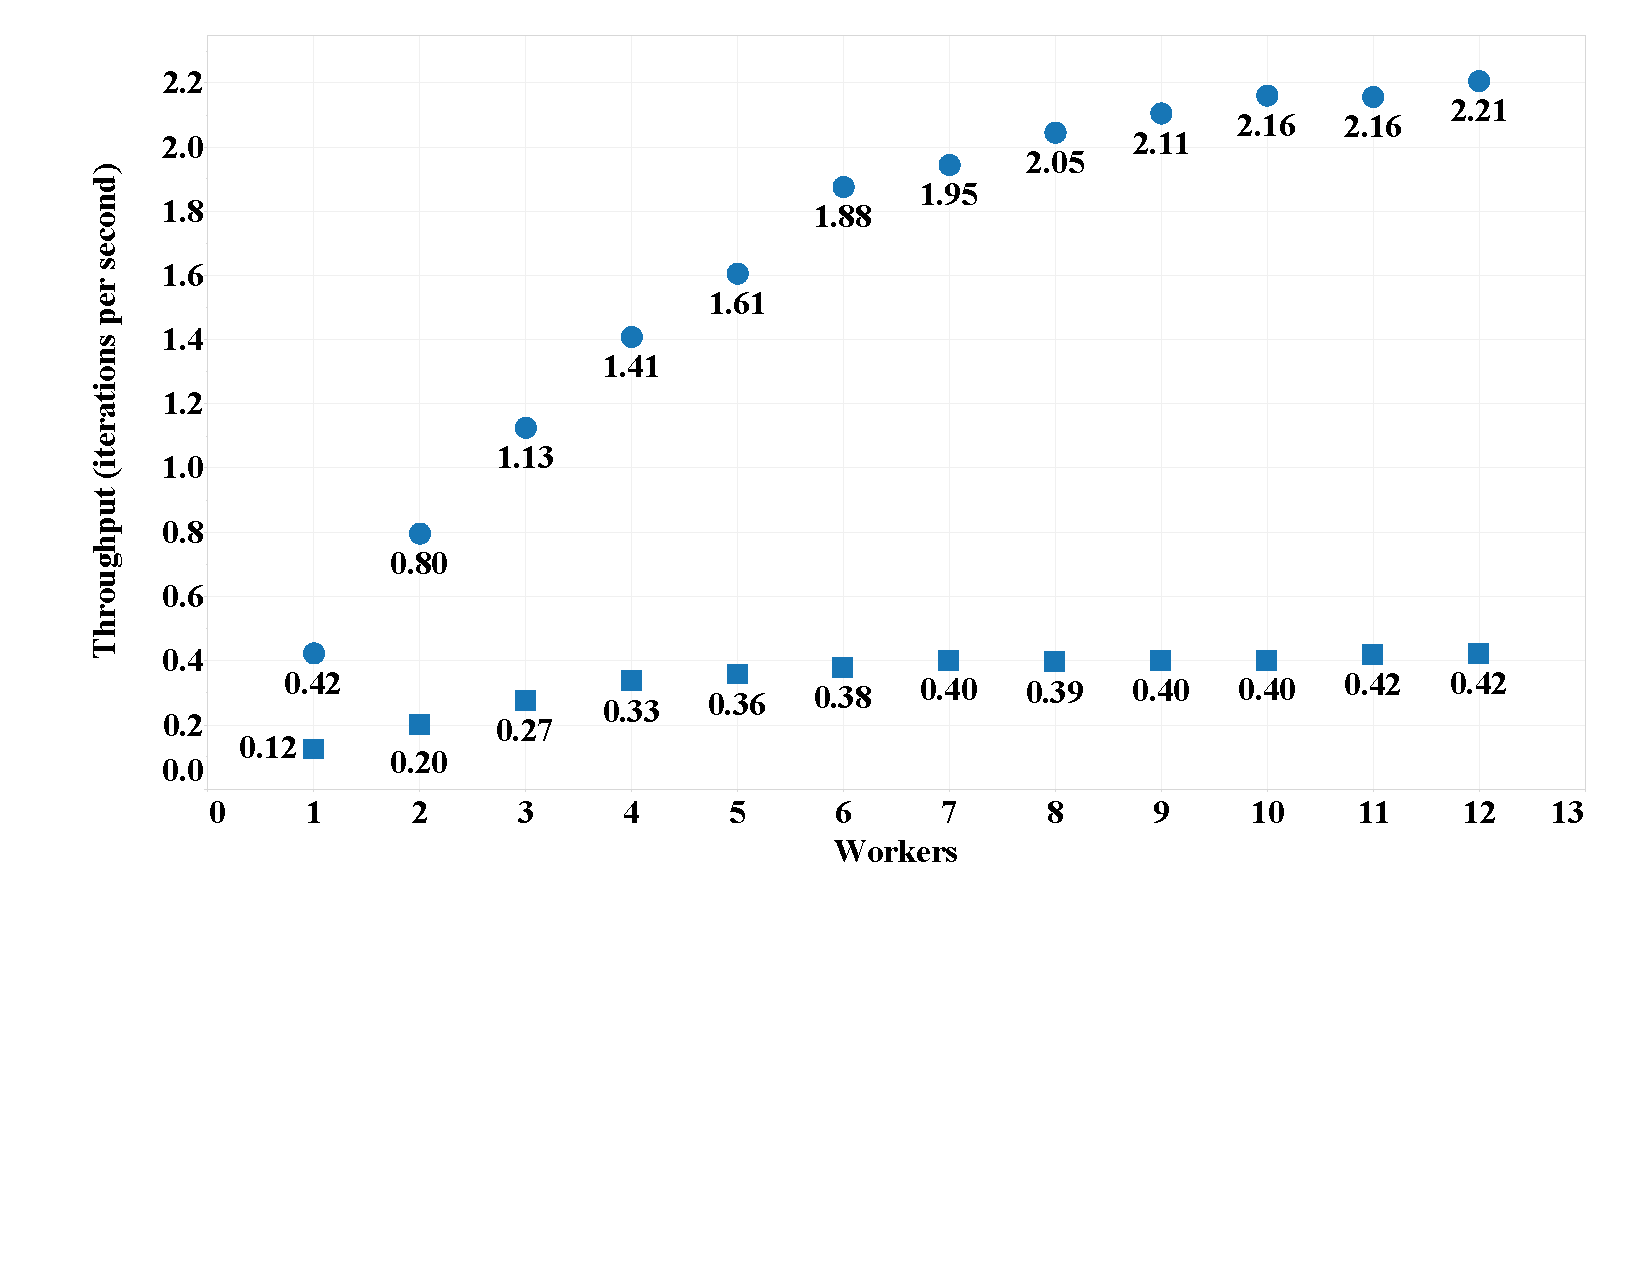
\includegraphics[width=5in,clip,trim=1cm 6cm 0 0]{figures/scalability_bsp.pdf}
\caption{Scalability.}
\label{fig:scalability_bsp}
\end{figure}

\begin{figure}[h]
\centering
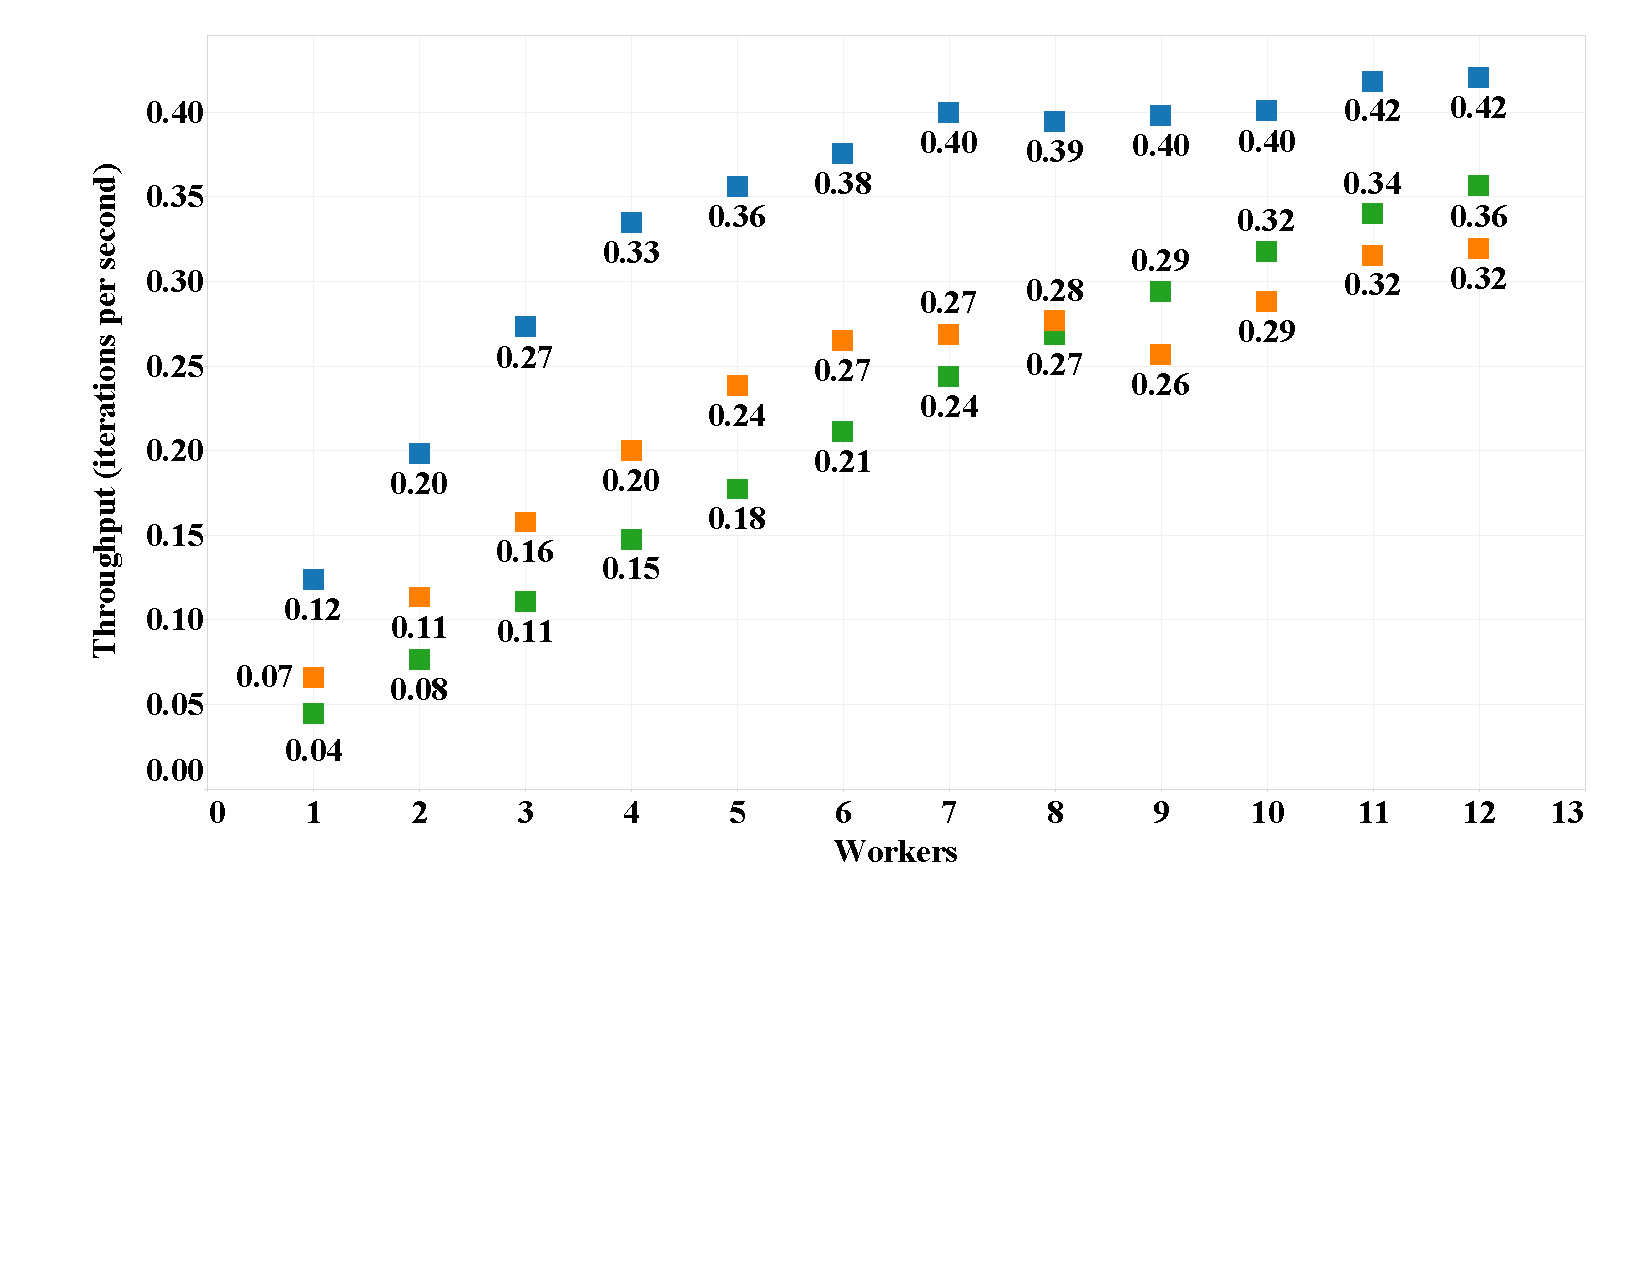
\includegraphics[width=5in,clip,trim=1cm 6cm 0 0]{figures/scalability_original.pdf}
\caption{Scalability.}
\label{fig:scalability_original}
\end{figure}

\begin{figure}[h]
\centering
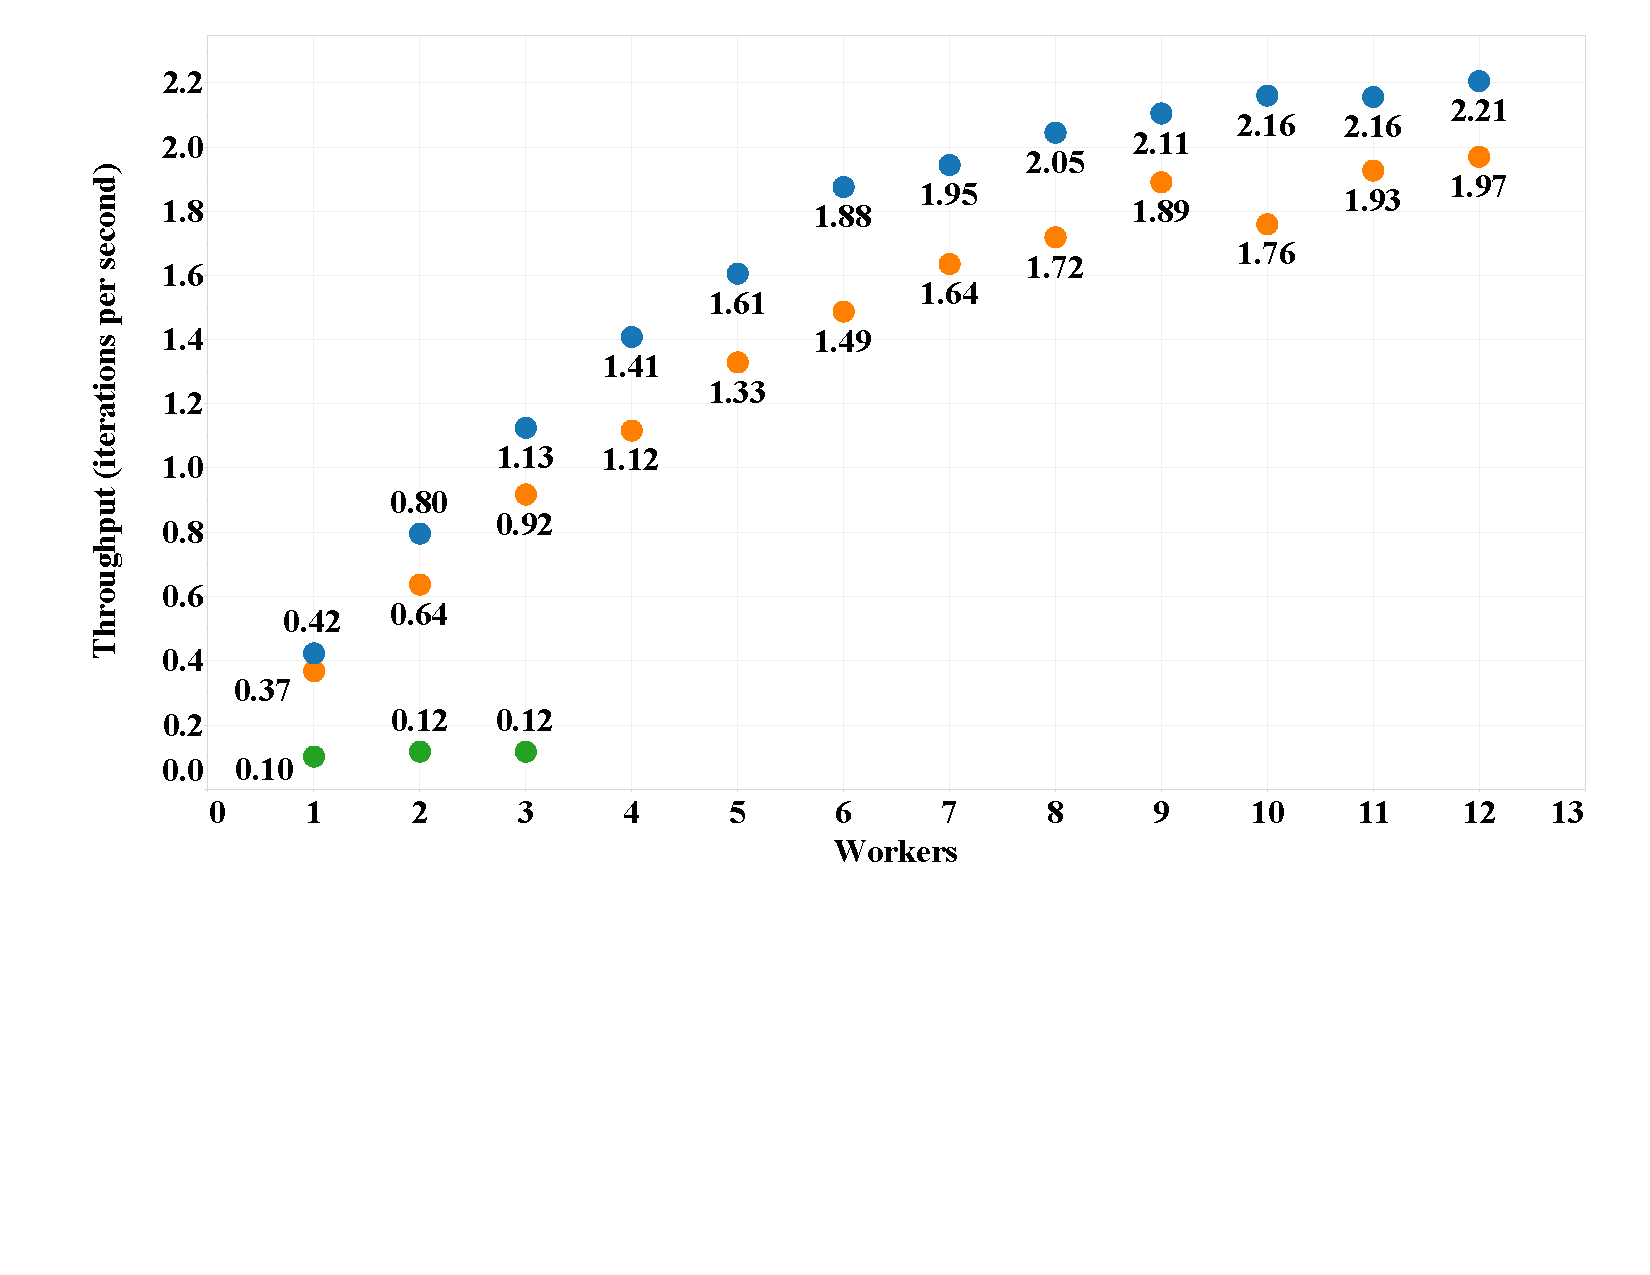
\includegraphics[width=5in,clip,trim=1cm 6cm 0 0]{figures/scalability_reordered.pdf}
\caption{Scalability.}
\label{fig:scalability_reordered}
\end{figure}

\begin{figure}[h]
\centering
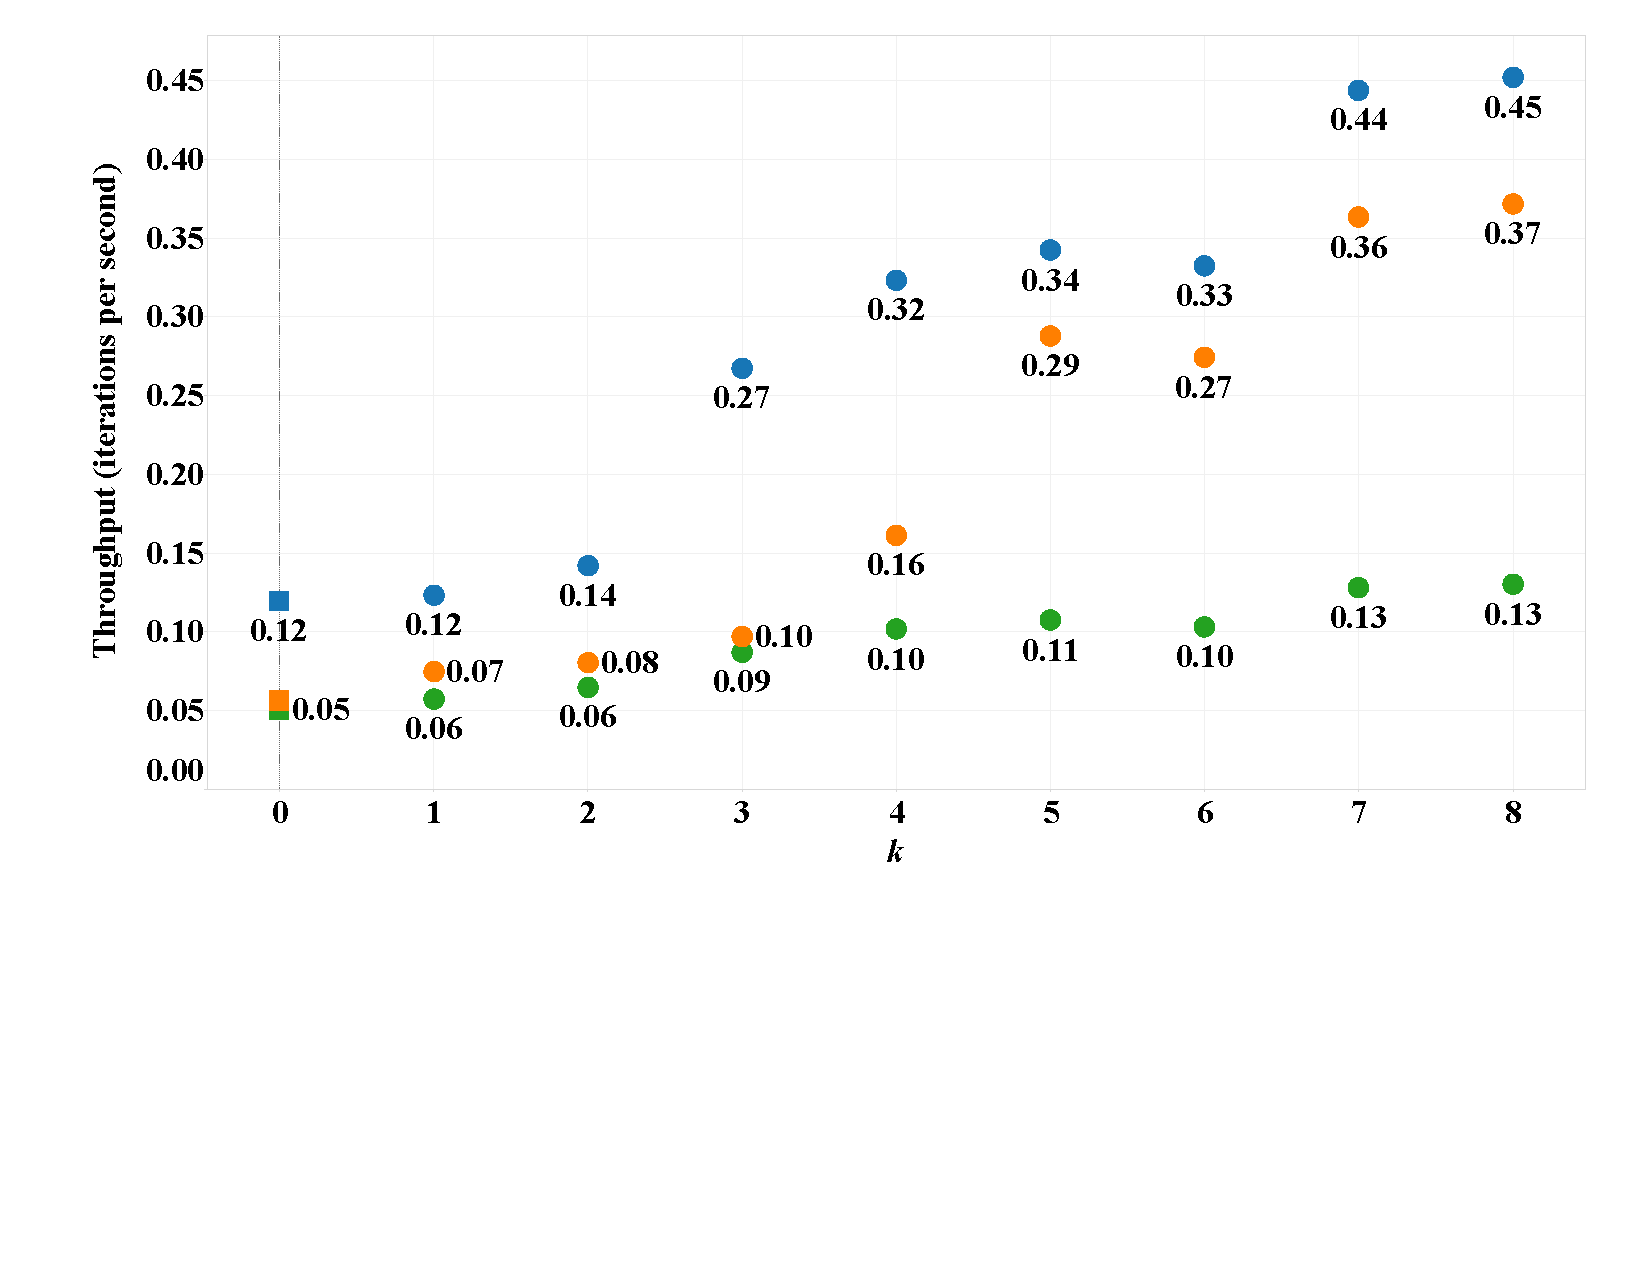
\includegraphics[width=5in,clip,trim=1cm 6cm 0 0]{figures/scalability_hilbert_bits_serial.pdf}
\caption{Scalability.}
\label{fig:scalability_hilbert_bits_serial}
\end{figure}

\begin{figure}[h]
\centering
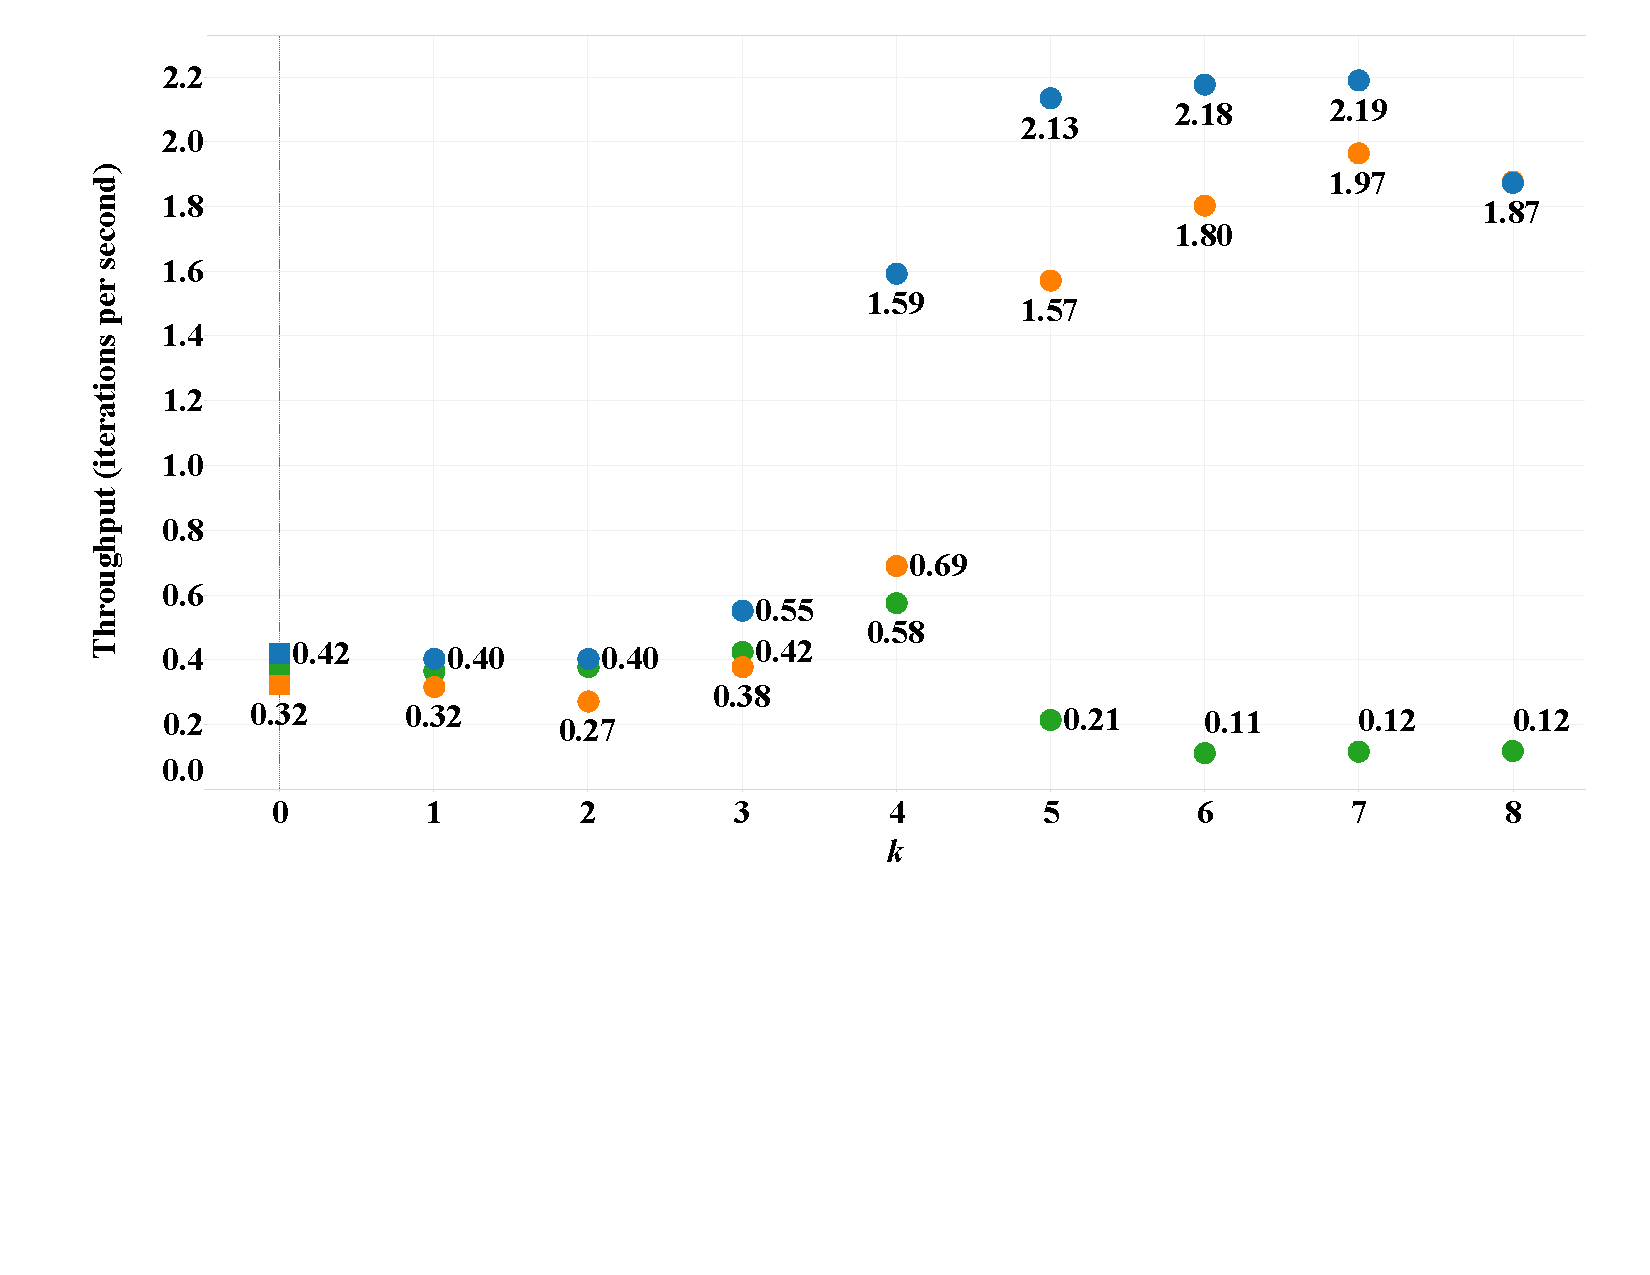
\includegraphics[width=5in,clip,trim=1cm 6cm 0 0]{figures/scalability_hilbert_bits_parallel.pdf}
\caption{Scalability.}
\label{fig:scalability_hilbert_bits_parallel}
\end{figure}



Once we have a good vertex partitioning and a strategy for distributed execution, throughput depends largely on single-machine performance. We explore a number of schemes to this end.


\subsection{Graph Representation in Memory}
We represent graphs in memory on a single machine as follows. We have an array of vertices and an array of edges. Each vertex contains data and a pointer into the edge array indicating the start of its list of edges. Adjacent vertices have adjacent edge lists. Each edge is simply a pointer into the vertex array. This organization is shown in Figure 3.

\subsection{Scheduling for Parallel Execution}
There are two major strategies for scheduling vertices for parallel execution that preserve the appearance of a global ordering across updates and avoid data races. The first is coloring \cite{KalerHaSc14}. If we color a graph so that no two neighboring vertices have the same color, we can safely execute the updates for vertices of the same color in fully in parallel. The reason is that if any vertex's data is being written by some thread, it cannot be read in parallel by another thread because this would require a neighbor of this vertex to be updating concurrently, which is impossible. With the coloring strategy, we sort the vertex array (and the corresponding edge lists) by color and step sequentially through the colors, updating the vertices of each color in a parallel loop.

The other strategy is priority DAG scheduling \cite{JonesPl93}. This involves assigning each vertex a distinct priority, so that we can form a DAG from our graph by adding a direction to each edge such that the source is the endpoint vertex with higher priority. We assign each vertex a counter equal to the number of predcessors it has. We can start by executing all vertices with no predecessors in parallel. Once a vertex is complete, we atomically decrement the counter of each of its successors. If a vertex's counter becomes zero, we can spawn the update of this vertex as another parallel strand of execution. We thus attain fairly high parallelism at the cost of using atomics, which can involve expensive memory barriers on modern hardware. Once again, there can be no data races because two neighboring vertices cannot execute concurrently since one must be the predecessor of the other.

\subsection{Achieving Cache Locality}
If we update the vertices in the vertex array sequentially, as we do with coloring-based scheduling, we get good cache locality (cached lines are processed completely after being fetched) on our accesses to the vertices being updated and to their corresponding entries in the edge array, which is also processed sequentially. Cache locality here includes data cache and TLB locality, since pages in the vertex and edge arrays corresponding to vertices being updated are processed completely after their first access. TLB misses have been shown to be a significant factor in the runtimes of data-intensive computations and are an important consideration for us.

While we get good locality on edge and vertex array accesses for vertices being updated, we get poor locality for accesses to the vertex array to fetch these vertices' neighbors. These accesses are essentially random unless we have sorted the vertex array in some locality-improving manner. Ideally we could store vertices' neighbors close to them in the vertex array. This would confer two benefits. First, TLB misses would fall since neighbors of a vertex will in most cases be stored in the same page as the vertex. Secondly, if a vertex being updated pulled neighbors that were yet to be updated into cache, those neighbors would be updated before they left cache, reducing cache misses.

These considerations suggest that ordering vertices in the vertex array by breadth-first search (BFS) level would be helpful. A vertex at BFS level $n$ can only have neighbors at BFS levels $n-1$ and $n+1$; if there was a neighbor at a smaller level, the vertex would have smaller level than $n$, and there can be no neighbors at levels greater than $n+1$ if the vertex is at $n$. Thus, if BFS levels are fairly small, ordering the vertices by BFS level would result in nearby neighbor accesses as desired. BFS levels are generally bounded in size in mesh graphs; they grow at first, but once the largest cross-section of the mesh is reached, successive levels should have similar size. The problem with ordering the entire vertex array by BFS level is that there are no longer defined sequential regions over which parallel update loops can be run -- since any two adjacent vertices could be neighbors -- so parallelism is lost. We implement and evaluate a hybrid coloring-BFS approach that restores some parallelism while preserving our locality wins: within each BFS level, we sort by color, so that within each BFS level we can update the vertices of each color in parallel. The BFS levels are executed sequentially. This scheme brings up an important point about the locality-parallelism design space -- after a point, increasing parallelism is not necessarily important. If there is enough parallelism to saturate the cores of the available machines, locality is likely the parameter worth optimizing.

% Analyze for priority DAG case
In the case of priority DAG scheduling, cache behavior is very different. We lose the locality of access to the vertex and edge arrays for vertices being updated that we have in the sequential processing case. But we are not without victories: when we update the last predecessor of some node we immediately afterwards update that node, at which point is hot in cache. So accesses to neighbors of vertices being updated do not have worst-case cache behavior as they do in the sequential processing case.

For ideal cache behavior, the story is similar to the sequential processing case. We would like for neighborhoods of nearby vertices to be stored fairly contiguously in the vertex array so that accesses to neighbors of vertices being updated tend not to cause TLB misses. We would also like these neighborhoods to be updated completely in some small time window so that fetched neighbors are updated before they leave cache. Achieving the first objective is possible by using a BFS-based ordering or by preserving the Z-number ordering described above for partitioning vertices across machines. We take the second approach because BFS levels may be larger than memory pages and therefore TLB misses are more likely under the BFS-based ordering. Achieving the second objective is much harder with DAG scheduling because the order in which vertices are updated is unclear. However, if we assign each vertex a priority equal to its Z-number, we suspect that if we spawn off the processing of vertices with no predecssors in order of Z-number and if we can assume that earlier spawned routines tend to execute to completion before later spawned routines begin executing (as is the case in the Cilk model of multithreading), then contiguous regions of the physical mesh should be processed nearly to completion in small periods of time. 

% "small period of time" is not precise...

%Draw parallel to cache-oblivious?

\subsection{Considering Parallelism}
% atomics, barriers in the priority DAG case
% cache transfers across processors are fast -- so as long as the data is in some cache, we are OK (not for TLB though) ... BUT
% Cilk -- steals high in the tree

\subsection{Prefetching}

\section{Graph Partitioning for Distributed Memory}
\label{sec:partitions}


Outline:
\begin{itemize}
\item Rationale for why Hilbert ordering should be good for distributed memory
\item Show fraction of edges that cross partitions w/ and w/o Hilbert ordering
\end{itemize}

\begin{figure}[h]
\centering
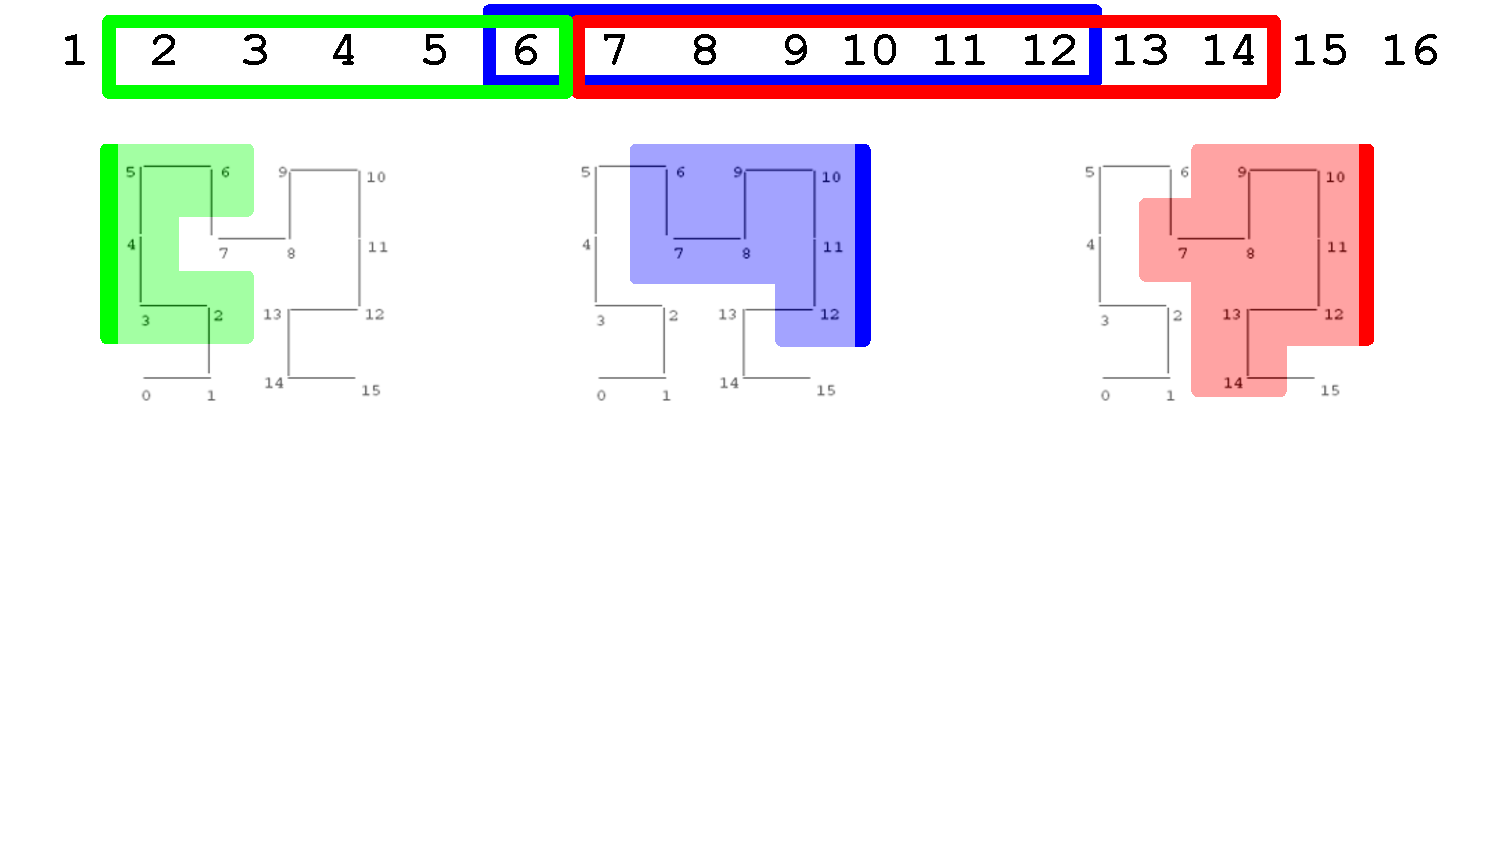
\includegraphics[width=5in,clip,trim=0 5cm 0 0]{hilbert_compact.pdf}
\caption{Examples of how contiguous subintervals yield compact
spaces in 2-dimensional space.}
\label{fig:hilbert_compact}
\end{figure}

\begin{figure}[h]
\centering
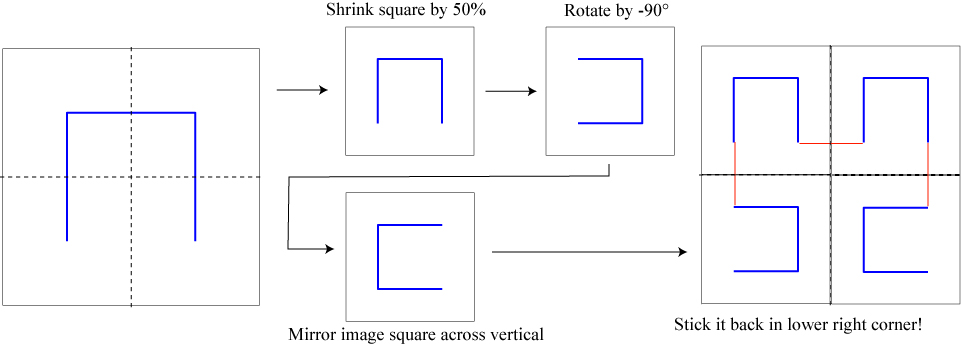
\includegraphics[width=5in,clip,trim=0 0 0 0]{fourthifs.jpg}
\caption{The construction of the Hilbert curve makes it
clear that contiguous subintervals of the curve yields
compact volumes in $N$-dimensional space: the curve always
makes 90 degree turns in an $N$-dimensional construction,
thus every pair of adjacent volumes in the Hilbert curve share a
face.}
\label{fig:hilbert_construction}
\end{figure}



In this section, we will describe how the Hilbert curve is also
a convenient mechanism for paritioning locally connected graphs
that are embeddable in a low-dimensional space.  That is, it 
generates a partition with small edge cuts.  We will discuss how
the priority-dag scheduling approach enables us to decompose the 
problem into two phases.  The first phase is to extend \proc{Prism}
to support a reshuffling operator, given a priority value from each
vertex, which re-organizes the graph data structure in linear order 
according to the priority function.  The second phase is to partition
the $n$ vertices by merely assigning $n/p$-sized compact subintervals
of vertices to each of the $p$ multi-core nodes.  Finally, we 
will describe the software architecture that integrates MPI commands
communicating over edges spanning partitions with the priority-dag 
scheduled computations on each multi-core node.  We will test the
performance of our implementation by measuring strong-scaling
performance on a small set of test graphs.


\section{Dealing with Distributed Execution}
Since an update function can only be run on a vertex if its 
neighbors are at most one iteration behind, we need to incur 
network traffic on every iteration to communicate vertex values 
for edges that cross machines. This can be done in a few ways. 
First, when an update function is being run on a vertex, it can 
fetch the values for neighbors on different machines and then 
run the necessary computation. This synchronous approach seems 
less than ideal, since the network traffic falls on the critical 
path of the iteration -- it is very likely that vertices that 
are capable of being updated without any network requests are 
waiting idle as the network requests complete.

Thus, an asynchronous approach is generally preferable. Our 
approach is as follows. For each edge that crosses machines, 
we declare one endpoint vertex as the predecessor and the other 
as the successor. Once the predecessor is updated, it sends 
its value to the machine to which the successor is assigned. 
Once the successor has received values from all of its 
predecessors, it can be scheduled for execution. If our 
partioning of vertices across machines is good and there are 
many vertices on each machine that have no dependencies on 
external vertices and therefore can be scheduled at any time, 
then there will be minimal waiting for network messages. Our 
scheme ensures that we satisfy the constraint that vertex 
updates must appear to be processed in some global order -- 
in other words, both of the endpoints of an edge cannot be 
updated in some iteration based on the other's data from 
the previous iteration.

% \begin{figure}[!t]
% \centering
% 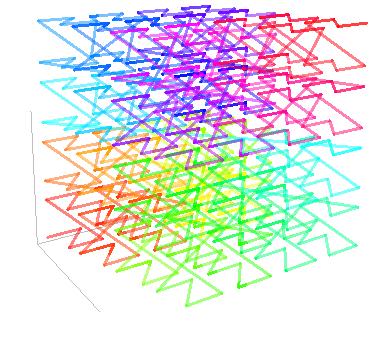
\includegraphics[width=2.5in]{z}
% \caption{A Z-order curve tracing out the 3D space bounded by the box.}
% \label{fig_z}
% \end{figure}

We partition vertices across machines using a technique 
based on space-filling curves. A 3D space-filling curve 
maps the real numbers to points in 3D space so that for 
an arbitrary point $p$ as we trace out more and more of 
the curve the distance from $p$ to the nearest point on 
the curve becomes smaller and smaller. We use a Z-order 
curve, which has the property that if two points on the 
curve are relatively close together, then the real numbers 
that generated those points tend to be relatively close. A 
Z-order curve in 3D space is shown in Figure 2.

Each vertex in a mesh graph can be assigned a particular 
coordinate in 3D space. Thus, we can draw a bounding box 
in 3D space around a mesh graph. We trace out a Z-order 
curve over a finite portion of its domain mapping to points 
n the bounding box. We then assign each vertex in the mesh 
to its nearest point in the traced curve and mark the vertex 
with the real number that generated this point, which we will 
call the Z-number. We then sort the vertices by Z-number. 
Nearby vertices in the sorted order should be nearby in the 
physical graph. We can then split this sorted list into 
contiguous chunks, one for each machine in our cluster. 
Since each chunk should correspond to some contiguous 
region in 3D space, the number of edges crossing machines 
should be fairly small, as explained in the previous section.

\section{Conclusion}
\label{sec:conclusion}




\bibliographystyle{acm}
\small\bibliography{allpapers}

\end{document}
